\documentclass[border=2cm]{standalone}
\usepackage{tikz}
\usetikzlibrary{calc}
\usetikzlibrary{angles,quotes}
\begin{document}
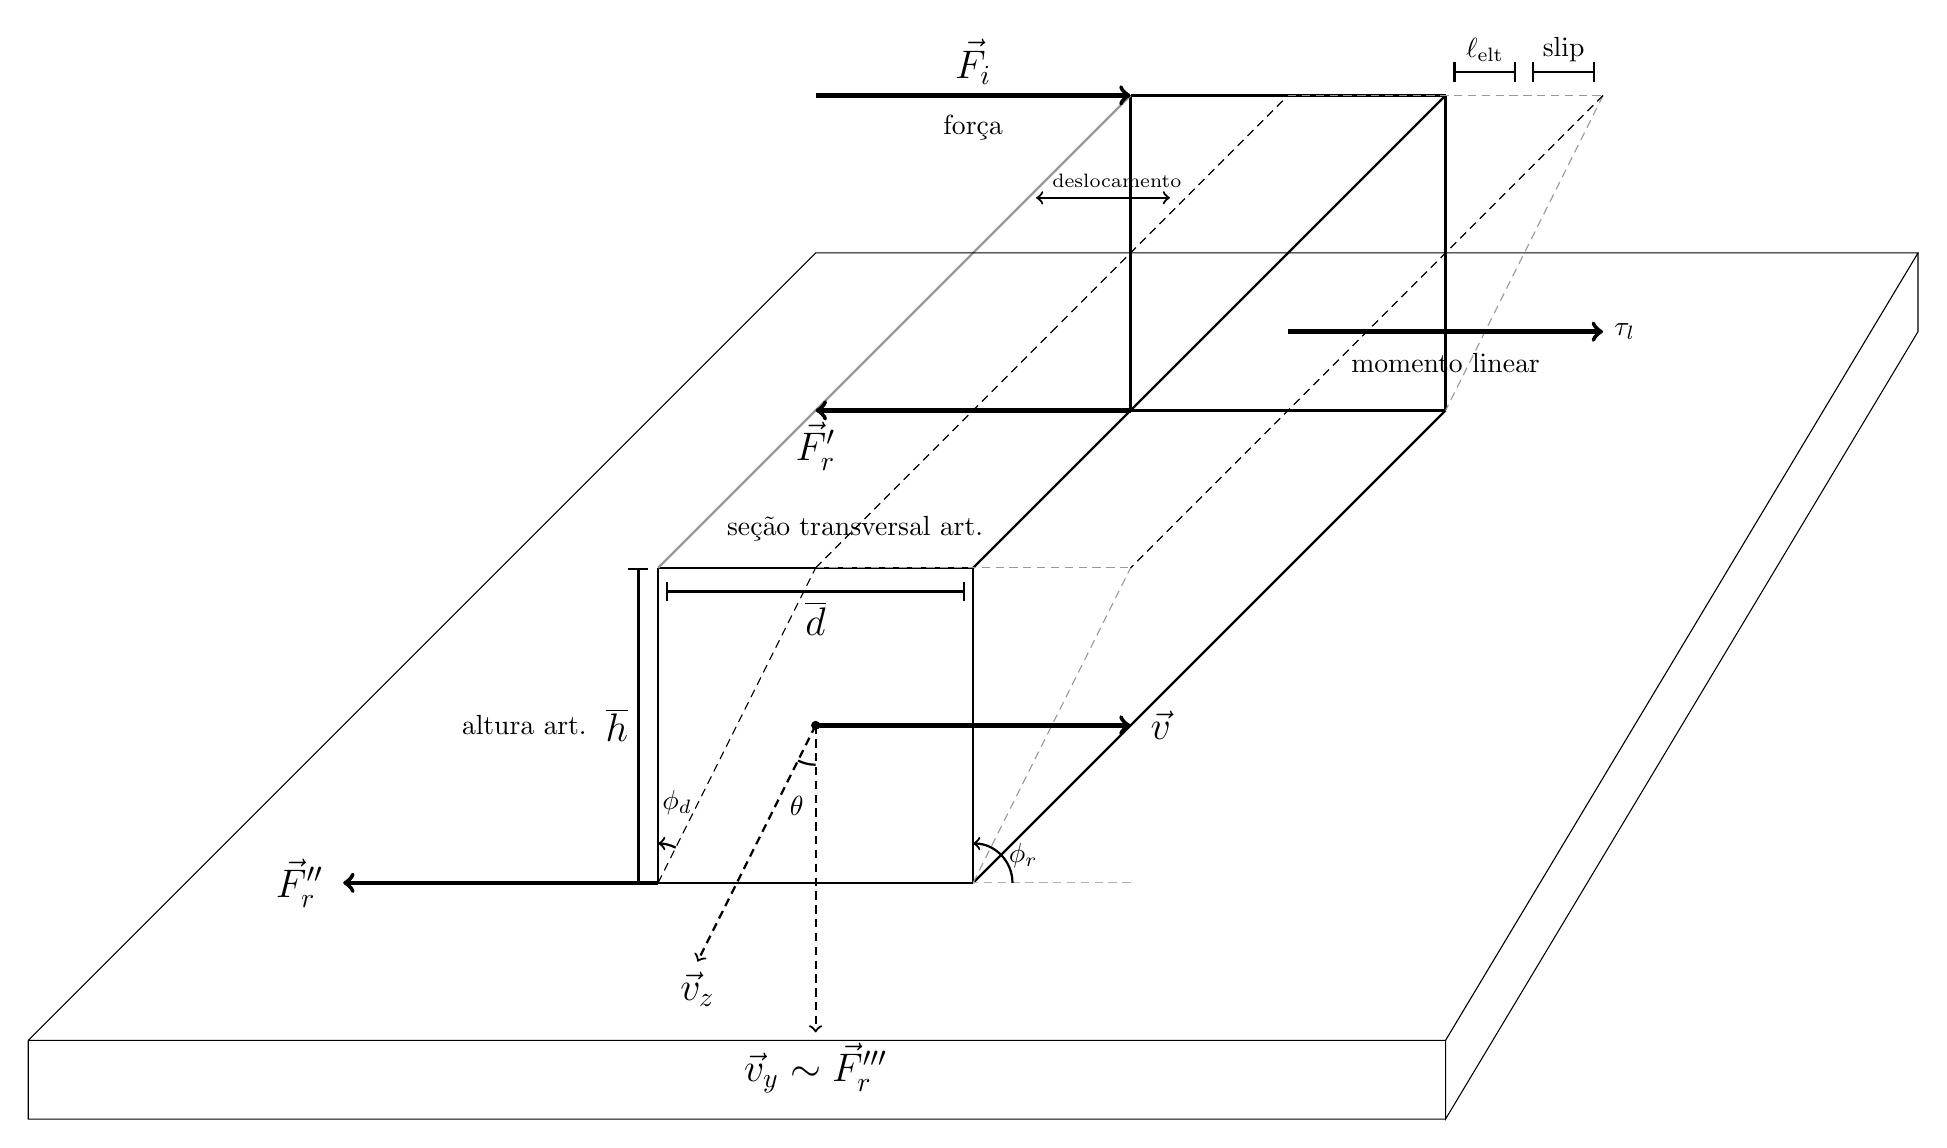
\begin{tikzpicture}

%\draw [help lines,step=.2] (-10cm,-10cm) grid (10cm,10cm);

	%%% shape
    \coordinate (C) at (0,0);
    \draw [fill=black] (C) circle (0.05cm);
    
    \coordinate (A1) at (-2,-2);
    \coordinate (A2) at (2,-2);
    \coordinate (A3) at (2,2);
    \coordinate (A4) at (-2,2);

    \draw[thick] (A1) -- (A2);
    \draw[thick] (A2) -- (A3);
    \draw[thick] (A3) -- (A4);
    \draw[thick] (A4) -- (A1);

    \coordinate (B1) at (4,4);
    \coordinate (B2) at (8,4);
    \coordinate (B3) at (8,8);
    \coordinate (B4) at (4,8);

    \draw[thick] (B1) -- (B2);
    \draw[thick] (B2) -- (B3);
    \draw[thick] (B3) -- (B4);
    \draw[thick] (B4) -- (B1);

    %\draw[densely dashed, gray!80] (A1) -- (B1);
    \draw[thick] (A2) -- (B2);
    \draw[thick] (A3) -- (B3);
    \draw[thick,gray!80] (A4) -- (B4);

    \coordinate (C1) at (0,2);
    \coordinate (C2) at (4,2);
    \coordinate (C3) at (0,2);
    \coordinate (C4) at (3,5);
    \coordinate (C5) at (6,8);
    \coordinate (C6) at (10,8);
    \coordinate (C7) at (8,4);
    \coordinate (C8) at (9,8);
    \coordinate (C9) at (3,2);
    \coordinate (C10) at (2,-2);

    \draw[densely dashed] (A1) -- (C1);
    \draw [densely dashed, gray!80] (A2) -- (C2);
    \draw[densely dashed, gray!80] (C1) -- (C2);
    \draw[densely dashed] (C3) -- (C4);
    \draw[densely dashed] (C4) -- (C5);
    \draw[densely dashed, gray!80] (C5) -- (C6);
    \draw [densely dashed, gray!80](C6) -- (C7);
    \draw [densely dashed](C6) -- (C2);
    %\draw [densely dashed](C8) -- (C9);
   % \draw [densely dashed,very thick](C9) -- (C10);

    \draw [|-|, thick] (-1.9,1.7) -- (1.9,1.7) node[midway, below] {\Large $\overline d$};
    \draw [|-|, thick] (-2.25,-2) -- (-2.25,2) node[midway, left] {\Large $\overline h$};
    \draw [|-|, thick,black] (9.9,8.3) -- (9.1,8.3) node[midway, above] {slip};
    \draw [|-|, thick,black] (8.9,8.3) -- (8.1,8.3) node[midway, above] {$\ell_{\mathrm{elt}}$};

    \draw [<-, ultra thick, scale=1] (4,8) -- (0,8) node[above, midway] {\Large $\vec F_i$};
    \node at (2,7.6) [black] {força};

    \draw [->, ultra thick, scale=1] (4,4) -- (0,4) node[below] {\Large $\vec F_{r}^{\prime}$};

    \draw [->, densely dashed, scale=1,thick] (0,0) -- (0,-3.9) node[below] {\Large $\vec v_{y} \sim \vec{F}_{r}^{\prime \prime \prime}$};

    \draw [->, densely dashed, scale=1,thick] (0,0) -- (-1.5,-3) node[below] {\Large $\vec v_{z}$};
    

    \draw [->, ultra thick, scale=1] (0,0) -- (4,0) node[above, midway, right=60] {\Large $\vec v$};
    \node at (8,4.6) [black] {momento linear};

    \draw [->, ultra thick, scale=1] (-2,-2) -- (-6,-2) node[above, midway, left=60] {\Large $\vec {F}_{r}^{\prime \prime}$};
    

    \draw [<->, thick] (2.8,6.7) -- (4.5,6.7) node[midway, right=5, above] {\scriptsize deslocamento};

    \node at (-3.7,0) [black] {altura art.};
    \node at (0.5,2.5) [black] {seção transversal art.};

% surface 

    \draw [black] (-10,-4) -- (8,-4) --++ (6,10) --++ (-14,0) --++ (-10,-10);
    \draw [black] (-10,-4) --++ (0,-1) --++ (18,0) --++ (0,1) --++ (0,-1) --++ (3,5) --++ (3,5) --++ (0,1);
    \draw[ultra thick, ->] (6,5) -- (10,5) node[right] {$\tau_l$};

% angles

    \coordinate (G1) at (4,-2);
    \coordinate (G2) at (2,-2);
    \coordinate (G3) at (2,2);
		
		%Angle
    \draw[dashed,gray!60,densely dashed] (G1) -- (G2);
	\pic[draw, ->, thick, "$\phi_r$", angle eccentricity=1.8, radius=1.3cm, below] {angle = G1--G2--G3};

    \coordinate (G4) at (-2,0);
    \coordinate (G5) at (-2,-2);
    \coordinate (G6) at (-1,0);

    \coordinate (G7) at (0,-2);
    \coordinate (G8) at (-1,-2);
    \pic[draw, ->, thick, "$\phi_d$", angle eccentricity=2.1, radius=1.7cm, midway] {angle = G6--G5--G4};
    \pic[draw, -, thick, "$\theta$", angle eccentricity=2.1, radius=1.7cm, midway] {angle = G8--C--G7};
    
  

\end{tikzpicture}
\end{document}